\chapterOrPart{Results}\label{ch:results}

\begin{explanation}
    It is mandatory to report the obtained results from modelling work, calculations, simulations and experiments.
    
    The guidelines for formatting figures, tables and mathematical expressions can be found in the appendix on formatting.
    
    Feel free to alter the name of the chapter and/or the sections.
\end{explanation}

% The framing of this chapter follows directly from the validation posture established in \Cref{sec:validation}: the model supports exploratory scenario comparison and stress testing, not calibrated national forecasting. Results are therefore reported as conditional projections under the four scenario-tree dimensions of \Cref{sec:scenarioTreeSystem}, each with a stable \texttt{scenario\_leaf\_id} that can be traced back to its configuration, inputs, and code state. Where the underlying artefact carries a quality caveat, the caveat is reported alongside the number.


\section{Final Model}
\label{sec:finalModel}

The final model used in this thesis is Model v3: a stochastic, physics-informed bottom-up residential demand model with explicit carrier accounting, PV and EV modules, and scenario-tree provenance. The model design enumerates a full four-dimensional scenario space of $2800$ leaves, but the thesis results are based on the executed subset available in the run registries. This distinction is important: the tree defines the reproducible experiment space, whereas only executed leaves constitute numerical evidence in this chapter.


\subsection{Canonical Execution Sets}
\label{sec:resultConfigs}

Three execution sets are used; as listed in \Cref{tab:canonical_configurations}. The first is the canonical thesis configuration, used for the annual baseline and validation runs under the 2023 historical-weather configuration. The second is the main scenario-tree ledger under \texttt{experiments/scenario\_tree}, which provides full-window climate-only comparisons for the current/frozen-stock technology cases. The third is the \texttt{scenario\_tree\_output34} design-year execution set, which provides stochastic hourly cohort runs for selected peak, diversity, and technology-stress comparisons.

\begin{table}[ht]
  \centering
  \footnotesize
  \caption{Executed model configurations used in the results chapter.}
  \label{tab:canonical_configurations}
  \begin{tabular}{@{}p{0.22\linewidth} p{0.23\linewidth}
                  p{0.23\linewidth} p{0.23\linewidth}@{}}
    \toprule
    \textbf{Setting} & \textbf{Validation config}
      & \textbf{Main scenario tree} & \textbf{Scenario set} \\
    \midrule
    Main artefact
      & \texttt{config/thesis.yaml}
      & \texttt{scenario\_tree}
      & \texttt{scenario\_tree\_output34} \\
    Purpose
      & baseline and validation checks
      & climate-only scenario comparison
      & peak, diversity, and technology-stress comparison \\
    Weather / climate
      & RMI/PVGIS 2023
      & processed CORDEX windows
      & selected CORDEX design years \\
    Active timestep
      & hourly
      & native daily CORDEX cadence
      & hourly; daily CORDEX forcing forward-filled \\
    Household treatment
      & $N=30$ for cohort validation; deterministic annual baseline where applicable
      & stock-weighted archetype / summary ledger
      & stochastic cohort, $N=30$ \\
    Executed evidence
      & full-horizon validation artefacts
      & $100$ latest-successful leaves
      & $80$ latest-successful leaves \\
    Technology coverage
      & current thesis stock
      & current/frozen stock
      & current, frozen, moderate electrification, high electrification + PV + EV \\
    \bottomrule
  \end{tabular}
\end{table}

\subsection{Experimental Coverage}
\label{sec:experimentalCoverage}

The scenario-tree schema enumerates $100$ historical baseline leaves and
$2700$ future leaves, for $2800$ leaves in total. The current thesis evidence consists of $180$ distinct latest-successful scenario leaves: $100$ leaves from the main \texttt{scenario\_tree} registry and $80$ leaves from the \texttt{scenario\_tree\_output34} registry. The main registry covers the baseline current-stock case and frozen-stock future controls across all three RCP pathways and all future climate windows with ten realizations per scenario group. The \texttt{output34} registry adds selected design-year stochastic cohort runs, including moderate and high electrification technology cases with five realizations per design-year group.
\newline The remaining leaves are part of the reproducible experiment design but are not used as executed evidence. Scenario results are therefore interpreted as a targeted exploration of climate and technology contrasts.

% \begin{table}[ht]
%   \centering
%   \footnotesize
%   \caption{Scenario-tree execution coverage used as numerical evidence.}
%   \label{tab:experimental_coverage}
%   \begin{tabular}{@{}l r r l@{}}
%     \toprule
%     \textbf{Registry} & \textbf{Enumerated space} &
%       \textbf{Latest-successful leaves} & \textbf{Role in thesis} \\
%     \midrule
%     \texttt{scenario\_tree}
%       & $2800$ leaves & $100$
%       & full-window climate-only comparison \\
%     \texttt{scenario\_tree\_output34}
%       & targeted design-year subset & $80$
%       & peak, diversity, and technology-stress comparison \\
%     \midrule
%     Combined executed evidence
%       & -- & $180$
%       & basis for scenario results reported in this chapter \\
%     \bottomrule
%   \end{tabular}
% \end{table}


\subsection{Validation Results}
\label{sec:resultValidation}

\Cref{tab:validation_results_summary} summarises the validation evidence used
to interpret the results. The table is deliberately conservative: calibration
checks, synthetic structural checks, measured-profile comparisons, and
technology-specific validation are not treated as equivalent forms of evidence.

\begin{table}[ht]
  \centering
  \footnotesize
  \caption{Validation headline metrics used to interpret the final model results.}
  \label{tab:validation_results_summary}
  \begin{tabular}{@{}p{0.20\linewidth} p{0.23\linewidth}
                  p{0.31\linewidth} p{0.18\linewidth}@{}}
    \toprule
    \textbf{Layer} & \textbf{Reference} &
      \textbf{Headline metric} & \textbf{Verdict} \\
    \midrule
    Annual baseline
      & Belgian annual targets / Eurostat shares
        \cite{eurostat_disaggregated_nodate}
      & Electricity \SI{3500}{kWh}; space-heating thermal
        \SI{15162}{kWh}; DHW thermal \SI{3000}{kWh};
        end-use share error $\approx 0$
      & calibration convergence\\
    Synthetic / Richardson
      & Richardson-style baseload
        \cite{Richardson2010CRESTElectricity}
      & synthetic Pearson $r=0.760$; synthetic diversity factor $3.22$;
        Richardson diversity factor $3.40$ vs $3.82$ reference
      & stochastic structure plausible; not Belgian empirical proof \\
    Smart-meter aggregate
      & Fluvius representative profiles \cite{Fluvius2024OpenData}
      & CVRMSE $\approx \SI{88}{\percent}$; Pearson $r \approx 0.40$;
        annual-energy error $\approx \SI{56}{\percent}$;
        peak-timing error $\approx 18$ h
      & failed external profile-shape check\\
    Smart-meter high-frequency
      & KU\,Leuven three-house case study \cite{KULeuven3House}
      & hourly model cannot reproduce household-level sub-hourly spikes
      & event-realism diagnostic; $N=3$ precludes population claim \\
    PV physical reference
      & PVGIS \cite{Huld2012PVGIS}
      & hourly $r=0.998$; hourly capacity-factor MAE $=0.011$;
        annual specific-yield error $\approx \SI{9}{\percent}$
      & strong physical-reference agreement \\
    PV country reference
      & Elia ODS032 \cite{Elia2024PVODS032}
      & daily capacity-factor correlation $r \approx 0.976$;
        monthly mean-absolute CF error $\approx \SI{25}{\percent}$
      & strong daily shape; monthly magnitude imperfect \\
    PV residential signature
      & Fluvius PV signature \cite{Fluvius2024OpenData}
      & mean-daily correlation $\approx 0.48$
      & moderate signature agreement \\
    EV residential signature
      & Fluvius EV signature \cite{Fluvius2024OpenData}
      & mean-daily $r=0.946$; peak hour \texttt{01:00};
        annual-energy gap $-\SI{43}{\percent}$, closing to
        $\approx -\SI{1}{\percent}$ under the \SI{2600}{kWh/yr} sensitivity
      & timing strong; magnitude requires sensitivity \\
    \bottomrule
  \end{tabular}
\end{table}

The resulting validation posture is mixed. Annual calibration and the PV and EV technology signatures justify using the model for conditional scenario experiments, but the unresolved Fluvius aggregate-profile mismatch means it cannot be presented as an externally calibrated Belgian smart-meter profile model. The scenario results that follow are therefore read as traceable conditional projections under the stated configuration rather than calibrated forecasts of Belgian residential load.


\pagebreak
\section{Climate Scenario Results}
\label{sec:climateScenarioResults}

This section reports the executed subset of the scenario tree. Climate-pressure and annual heating-change results draw on the 100 successful full-window leaves (daily cadence; ten realizations per scenario group); peak-load and grid-stress results draw on the 80 successful design-year leaves in \texttt{scenario\_tree\_output34}, which run hourly 30-household stochastic cohorts with five realizations per design-year group. Neither ledger includes active cooling final energy, so cooling is treated as a demand-pressure indicator only.


\subsection{Physical Impact}
\label{sec:physicalImpact}

The physical climate signal is isolated under \texttt{tech\_frozen\_stock},
which holds the dwelling and technology stock fixed so that changes in the
heating and cooling indicators reflect the imposed climate window and pathway
rather than electrification. \Cref{tab:climate_degree_days_results} reports
annualized HDD$_{18}$ and CDD$_{22}$ from the full-window summaries alongside
the paired annual useful-heating change.

\begin{table}[ht]
  \centering
  \footnotesize
  \caption{Climate-pressure and useful-heating response under the frozen-stock climate-only comparison. HDD$_{18}$ and CDD$_{22}$ are annualized degree-day means; useful-heating change is the paired annual mean from the full-window summary layer.}
  \label{tab:climate_degree_days_results}
  \begin{tabular}{@{}l l r r r r r@{}}
    \toprule
    \textbf{Window} & \textbf{Pathway} &
    \textbf{HDD$_{18}$} & $\Delta$\textbf{HDD$_{18}$} &
    \textbf{CDD$_{22}$} & $\Delta$\textbf{CDD$_{22}$} &
    $\Delta Q_{\text{heat}}$ \\
    & & ($^{\circ}$C d/yr) & (\%) & ($^{\circ}$C d/yr) & ($^{\circ}$C d/yr) & (\%) \\
    \midrule
    1981--2005 & historical & 3341 & +0.0 & 14.3 & +0.0 & +0.0 \\
    2030--2049 & RCP 2.6 & 3009 & -9.9 & 40.3 & +26.0 & -10.1 \\
    2030--2049 & RCP 4.5 & 3071 & -8.1 & 24.2 & +9.9 & -8.5 \\
    2030--2049 & RCP 8.5 & 3034 & -9.2 & 21.2 & +6.9 & -9.7 \\
    2050--2070 & RCP 2.6 & 3017 & -9.7 & 31.4 & +17.1 & -7.3 \\
    2050--2070 & RCP 4.5 & 2846 & -14.8 & 50.9 & +36.6 & -13.6 \\
    2050--2070 & RCP 8.5 & 2718 & -18.7 & 59.0 & +44.6 & -19.9 \\
    2080--2100 & RCP 2.6 & 3073 & -8.0 & 31.9 & +17.6 & -5.9 \\
    2080--2100 & RCP 4.5 & 2803 & -16.1 & 44.7 & +30.3 & -16.2 \\
    2080--2100 & RCP 8.5 & 2306 & -31.0 & 109.3 & +94.9 & -33.3 \\
    \bottomrule
  \end{tabular}
\end{table}

\subsubsection*{Change in degree days}
The strongest executed climate-pressure case is \texttt{long\_term\_2080\_2100} under RCP\,8.5. Relative to the historical baseline, HDD$_{18}$ falls from about $3341$ to $2306\,^{\circ}\mathrm{C}\cdot\mathrm{d}$ per year ($-31.0\,\%$; \Cref{fig:phase1_hdd_pct_heatmap}), while CDD$_{22}$ rises from $14.3$ to $109.3\,^{\circ}\mathrm{C}\cdot\mathrm{d}$ per year (\Cref{fig:phase1_cdd_abs_heatmap}). The pathway ordering is not monotonic in every near-future cell of this single GCM--RCM chain, so the robust statement is directional and conditional: warming reduces heating pressure and increases cooling pressure, with the largest response in the long-term RCP\,8.5 cell.

\begin{figure}[ht]
  \centering
  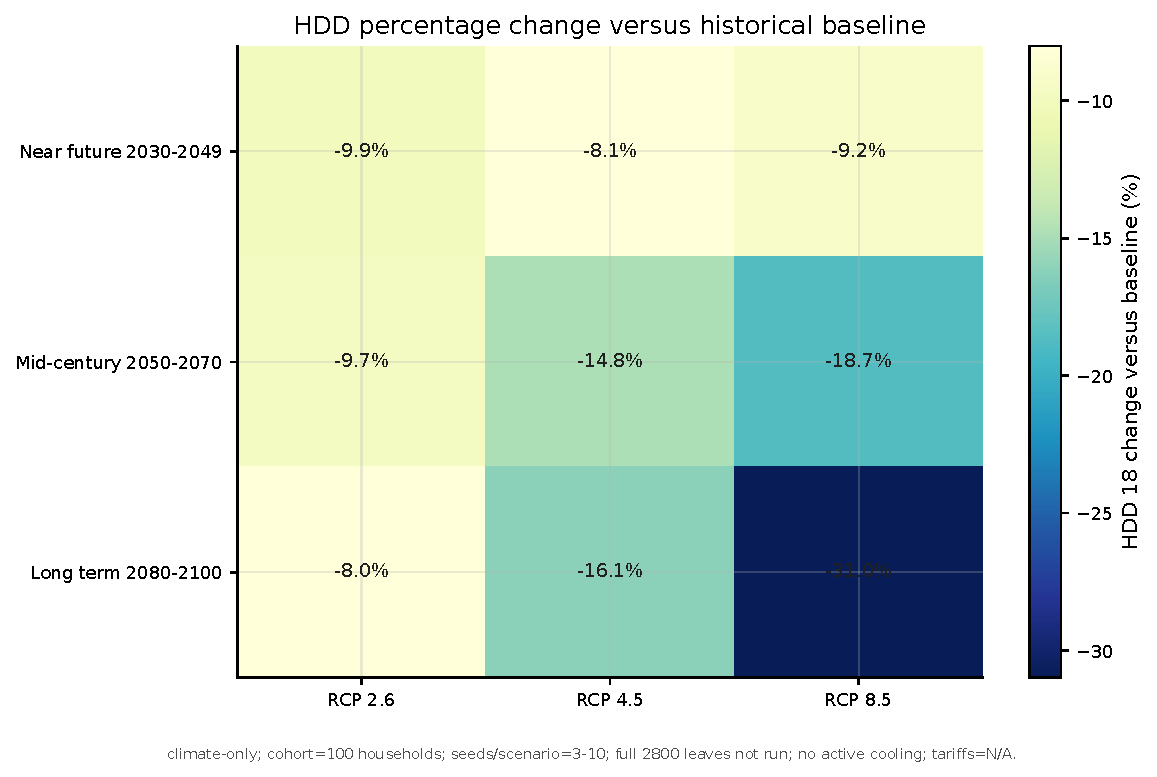
\includegraphics[width=0.8\textwidth]
    {figures/phase1_hdd_pct_decrease_heatmap.pdf}
  \caption{HDD$_{18}$ percentage decrease across climate window $\times$ RCP pathway, relative to the historical baseline window. The long-term RCP\,8.5 cell shows the strongest executed reduction, consistent with the $-31.0\,\%$ headline in \Cref{tab:climate_degree_days_results}.}
  \label{fig:phase1_hdd_pct_heatmap}
\end{figure}

\begin{figure}[ht]
  \centering
  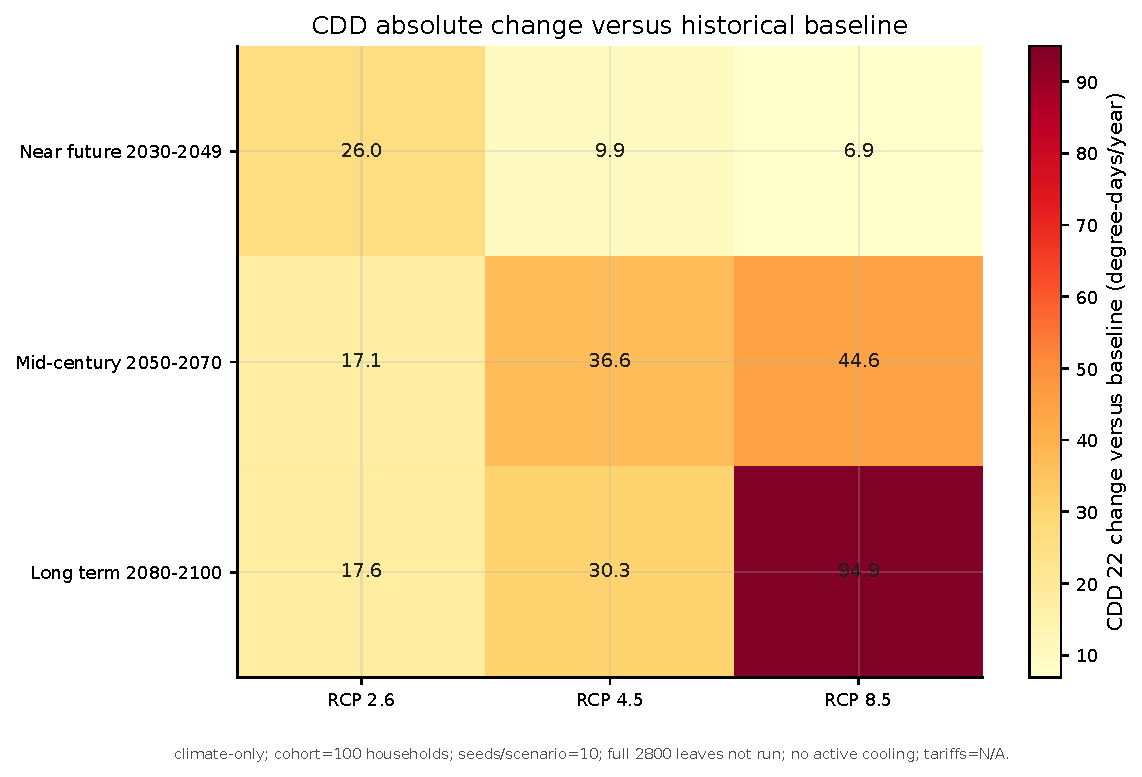
\includegraphics[width=0.8\textwidth]{figures/phase1_cdd_abs_increase_heatmap.pdf}
  \caption{CDD$_{22}$ absolute increase across climate window $\times$ RCP pathway, relative to the historical baseline window. CDD$_{22}$ rises from a small base; the long-term RCP\,8.5 cell reaches about $+94.9\,^{\circ}\mathrm{C}\cdot\mathrm{d}$ per year.}
  \label{fig:phase1_cdd_abs_heatmap}
\end{figure}

\subsubsection*{Useful heating demand}
The useful-heating response follows the same broad direction as HDD$_{18}$: all frozen-stock future cells reduce annual useful-heating demand relative to the paired historical baseline. The response is not perfectly ordered across all near-future pathway cells, which is expected for one regional climate-model chain and finite window samples. The strongest reduction again occurs in the long-term RCP\,8.5 cell, where useful heating falls by about $33.3\,\%$ in the full-window comparison (\Cref{fig:phase1_sh_pct_heatmap}).

\begin{figure}[ht]
  \centering
  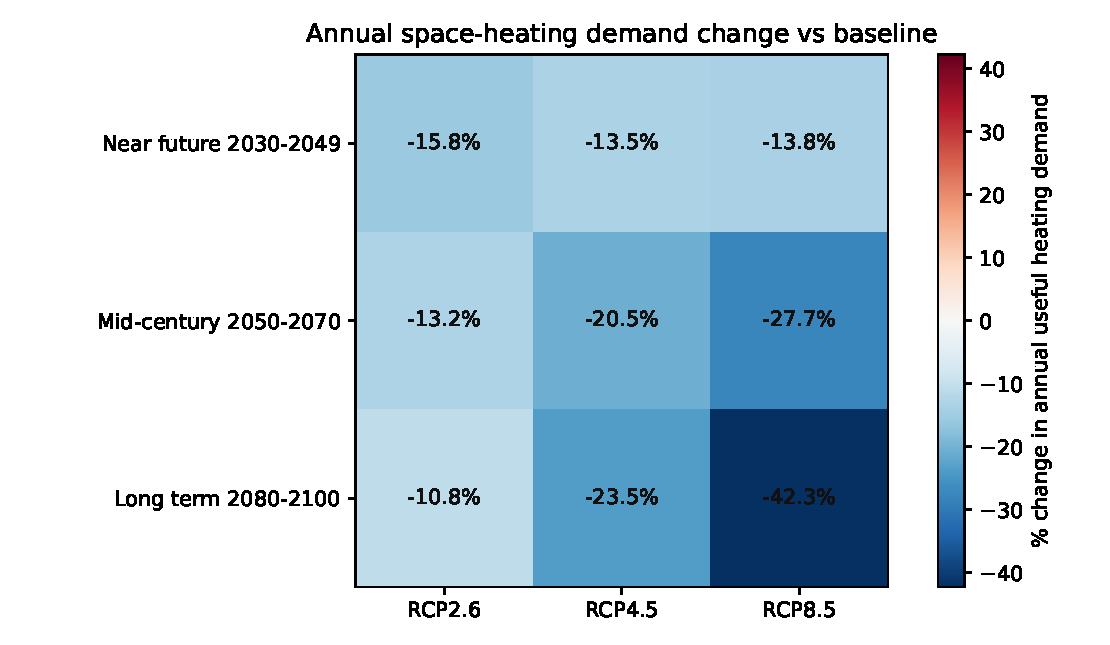
\includegraphics[width=0.8\textwidth]{figures/annual_space_heating_percentage_heatmap.pdf}
  \caption{Annual useful space-heating percentage change across climate window $\times$ RCP pathway under \texttt{tech\_frozen\_stock}. All executed future cells reduce useful-heating demand relative to the paired historical baseline, with the strongest reduction in long-term RCP\,8.5.}
  \label{fig:phase1_sh_pct_heatmap}
\end{figure}

\subsubsection*{Climate change physical results}
These results support a clear but limited conclusion. Climate change reduces modelled space-heating pressure under fixed stock, but the model does not translate higher CDD into active cooling electricity. The cooling result is therefore a demand-pressure result, not a forecast of cooling load.


\subsection{System Impact}
\label{sec:systemImpact}

Peak-grid results are taken from the hourly design-year runs because peak import, load duration and threshold exceedance are hourly quantities. \Cref{tab:peak_grid_import_results} reports the cold-design-year stress case for the historical baseline and the long-term RCP\,8.5 cases.

\begin{table}[ht]
  \centering
  \footnotesize
  \caption{Cold-design-year grid-stress results for the hourly 30-household runs.}
  \label{tab:peak_grid_import_results}
  \resizebox{\textwidth}{!}{%
  \begin{tabular}{@{}l l r r r r r@{}}
    \toprule
    \textbf{Technology case} & \textbf{Climate case} &
    \textbf{Grid import} & \textbf{Gas} &
    \textbf{Peak import} & $\Delta$\textbf{peak} &
    \textbf{Hours > threshold} \\
    & & (kWh/hh/yr) & (kWh/hh/yr) & (kW) & (\%) & (h/yr) \\
    \midrule
    \texttt{current\_stock} & baseline / historical & 5845 & 19406 & 30.80 & +0.0 & 1968 \\
    \texttt{frozen\_stock} & 2080--2100 / RCP 8.5 & 5249 & 13934 & 30.58 & -0.7 & 1424 \\
    \texttt{moderate\_electrification} & 2080--2100 / RCP 8.5 & 18497 & 9063 & 106.45 & +245.6 & 6985 \\
    \texttt{high\_electrification\_pv\_ev} & 2080--2100 / RCP 8.5 & 34285 & 1894 & 188.40 & +511.7 & 8760 \\
    \bottomrule
  \end{tabular}}
\end{table}

\subsubsection*{Peak grid import}
Across the executed design-year subset, technology choice dominates climate forcing for peak grid import. Under frozen stock, long-term RCP\,8.5 leaves the cohort peak almost unchanged ($30.80$ to $30.58$ kW), whereas switching the technology case under the same forcing lifts it to $106.45$ kW under moderate electrification and $188.40$ kW under high electrification with PV and EV.

\subsubsection*{Threshold exceedance}
The threshold-hour metric is a stress diagnostic relative to the configured cohort threshold rather than a prediction of distribution-grid failure. It remains informative: under the current threshold definition, the electrified cases exceed the historical stress band for most or all hours of the design year.


\subsection{Economic and Emissions Impact}
\label{sec:economicImpact}

The economic and emissions figures are conditional accounting outputs under the configured tariff, CAPEX and emission-factor assumptions, and should not be read as policy forecasts. 

\subsubsection*{Economics}
In the cold-design-year long-term RCP\,8.5 case, the dynamic-tariff bill falls from about € 4082 per household in the historical current-stock baseline to € 3351 under frozen stock, because gas demand falls with heating pressure. The same tariff raises bills to about € 6892 under moderate electrification and € 10965 under the high-electrification PV--EV case. Across the executed tariff scenarios, electrification remains more expensive under the current tariff, export-credit and capex assumptions; the current outputs therefore should not be framed as showing favourable electrification economics.

\subsubsection*{Emissions}
Operational emissions use a fixed electricity-emission factor. Under that assumption, frozen stock falls to about $3602$ kgCO$_2$/household/year ($-24.9\,\%$), moderate electrification falls slightly to about $4605$ kgCO$_2$/household/year ($-4.0\,\%$), and the high-electrification PV--EV case rises to about $5525$ kgCO$_2$/household/year ($+15.2\,\%$). This result is sensitive to the fixed electricity factor and should be interpreted as a scenario-accounting result, not as a general decarbonisation conclusion.


\subsection{Sensitivity and Uncertainty}
\label{sec:sensitivityStochasticRobustness}

The executed design-year scenario results contain five stochastic seeds per selected scenario/design-year group, and the comparison files report P10/P50/P90 bands across those seeds. The full-window climate-only results use ten paired realizations per scenario group.

The EV annual-energy sensitivity exists in the validation artifacts and shows that the base EV profile uses about $1491$ kWh per active EV per year versus a Fluvius-derived reference of about $2626$ kWh/year ($-43.2\,\%$), while the $2600$ kWh/year sensitivity closes the annual gap to about $-1.0\,\%$ without changing the mean-daily timing correlation. Scenario results involving \texttt{tech\_high\_electrification\_pv\_ev} should therefore be read as conditional on the configured EV charging magnitude.

Finally, all climate results remain conditional on the single CORDEX chain used here. The executed tree samples pathways, windows, technology cases and seeds, but it does not sample inter-model climate uncertainty.
\mode<all> % do not remove
